\documentclass[12pt]{scrartcl}

\title{fLaCPGA - FPGA fLaC Implementation}
\subtitle{Design Document}
\author{Emmanuel Jacyna - 24227498}
\date{\today}

\usepackage[T1]{fontenc}
\usepackage[utf8]{inputenc}

\setkomafont{disposition}{\normalfont\bfseries}
\usepackage{hyperref}
\usepackage{graphicx}
\usepackage{tabularx}
\usepackage{float}
\usepackage{amsmath}
\usepackage{listings}
\usepackage{pgfgantt}
\bibliographystyle{unsrt}


\begin{document}
\pagestyle{myheadings}
\markright{Emmanuel Jacyna\hfill 24227498\hfill}
  \maketitle
  \begin{figure}[H]
    \centering{\includegraphics[scale=1]{imgs/FLAC_logo_inverted.png}}
  \end{figure}
  
  \tableofcontents
  
  \section*{Abstract}
  The purpose of this document is to describe the design of the fLaCPGA project. It includes a detailed description of the fLaC format, a discussion of the goals and requirements of the project, and a look ahead into what will be achieved next semester.
  
  
  \section{Introduction}
  The goal of my final year project is to investigate hardware optimization techniques through the implementation of a Free Lossless Audio Codec (henceforth, fLaC) decoder and encoder in Verilog. fLaC is a lossless audio compression codec that is very popular as a method of distributing high quality audio recordings and for compressing large audio archives\cite{flac_popular}. 
  
  Whilst there are a number of software implementations of the fLaC encoder and decoder, targeted to both traditional microprocessors and digital signal processors (DSPs), there are no freely available ASIC or FPGA implementations. An efficient hardware implementation would be of great use for a number of reasons. Many nations are now in the process of digitising large national audio archives. These audio archives require data to be compressed losslessly in order to preserve content in a format faithful to the original, however, uncompressed lossless data consumes large amounts of space. Currently, uncompressed formats such as WAVE and BWF\_WAVE are quite popular for audio archiving\cite{pres_fmts}. 
  
  Compressed audio has the major benefit of reducing space usage by 50\% or more, potentially doubling an archive's potential storage space. In order to convert large (terabytes) amounts of audio data to a compressed format, a lot of computing power is required. A hardware decoder that performed better than a software decoder would reduce encoding time and potentially reduce power consumed by the encoding process. fLaC is also gaining popularity as a medium for portable audio players. These players are very sensitive to power consumption, thus a hardware implementation would be of great use in reducing the power load of the decoding process. Another potential use case of a hardware encoder would be in a recording studio. Instead of recording audio to an uncompressed format, high quality audio could be encoded in real time as it comes in.
  
  \section{Audio Compression Overview}
  Just as with general data compression, there are two main methodologies for compressing audio data, lossy and lossless. Lossy audio encoding most often includes techniques such as psychoacoustic compression, where sounds that humans cannot perceive or differentiate are removed from the audio\cite{principles_of_digital_audio}. These techniques will not be the focus of this project. Lossless compression, by comparison, encodes audio perfectly, that is, the decoded audio samples are identical to the original input samples. Lossless techniques are still affected by problems inherent to the digitization process such as quantisation noise and recording device noise, however they provide a faithful encoding of the original data.
  
   \begin{figure}[H]
    \centering{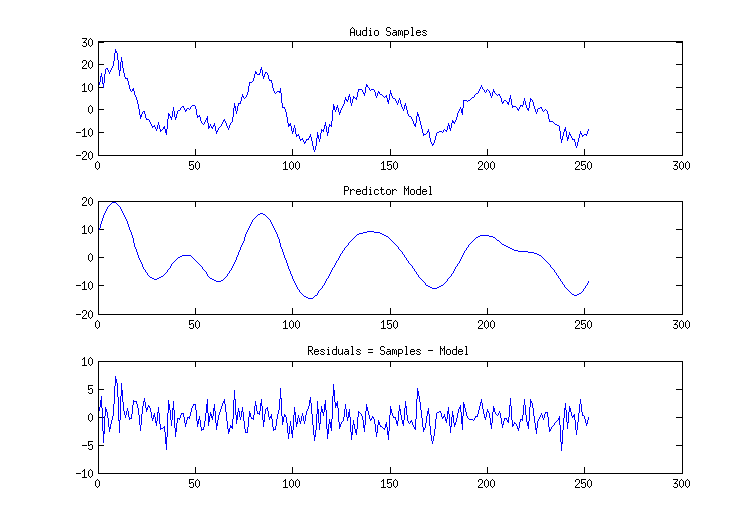
\includegraphics[scale=.8]{imgs/predictor_theory.png}}
    \caption{Predictor Concept}
    \label{fig:pred_theory}
  \end{figure}
  
  The main goal of any compression algorithm is to remove redundancy from data, thereby reducing the amount of information needed to reproduce the data. Audio data is often highly redundant, samples of data that are close to each other will usually have very similar patterns, for example, samples of a clarinet playing the same note for a number of seconds will clearly have a similar spectral pattern over the period of time the note is held, thus offering redundancy to be exploited. The most popular method for lossless compression of audio data is to find an accurate model of the audio (a \textit{predictor}), find the error (often called \textit{residuals}) between the predictor and the true audio, then to encode the residuals using a variable bit length encoding in order to increase the entropy of the signal\cite{lpc_model_comparison}. The coefficients of the model can then be used with the residuals to reconstruct the orginal signal.
  
  The fLaC lossless audio compression algorithm borrows heavily from prior work in lossless encoding including the Shorten algorithm\cite{shorten}, and the AudioPAK algorithm\cite{audiopak}. These algorithms use a technique called \textit{linear prediction} to produce their audio model, and use Golomb-Rice encoding to perform the entropy encoding phase of the compression. The advantage of these algorithms is the ease with which they can be translated into hardware, as the linear prediction step consists of a number of multiplies and adds, whilst the Golomb-Rice encoding consists of bit-shifting and unary encoding.
  
  \subsection{fLaC Overview}
  \subsubsection{fLaC Encoding Process}
  \begin{figure}[H]
    \centering{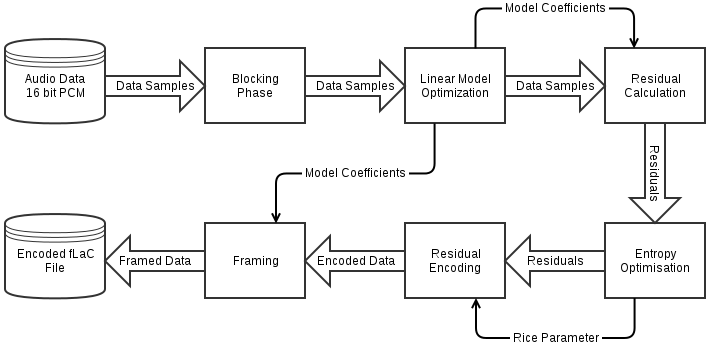
\includegraphics[scale=.8]{imgs/flac_encoding_overview}}
    \caption{Overview of fLaC Encoding Process}
    \label{fig:encoding_process}
  \end{figure}
  The fLaC encoding process consists of two major stages\cite{flac_format}. Finding a linear model that minimises the prediction error, and finding the best set of rice parameters to encode a block of residuals. As well as this, the output data must be framed appropriately and encoded using these optimal parameters before being output to a file/stream. Figure \ref{fig:encoding_process} gives an overview of the entire encoding process.
  
  \subsubsection*{Finding the best linear model}
  \begin{figure}[H]
    \centering{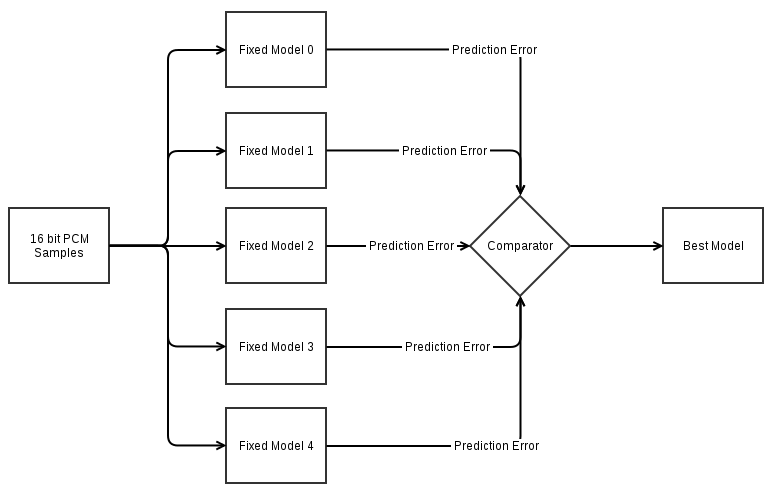
\includegraphics[scale=.8]{imgs/flac_fixed_overview}}
    \caption{Finding the best fixed model}
    \label{fig:fixed_optimisation}
  \end{figure}
  fLaC has two options for finding the best linear model. It can either choose from four precalculated predictors, the "fixed" predictors, or it can find a more accurate model using the autocorrelation of the audio signal to calculate the optimal predictor coefficients using the Levinson-Durbin recursion method\cite{levinson_durbin}. The fixed model has the advantage that it requires less computation to calculate, and it also results in a much smaller frame header size. The fixed model usually achieves around 50\% compression for most audio data. The Levinson-Durbin method has the advantage that the models it calculates are almost always more accurate than the fixed models, and thus will result in better compression ratios. Choosing the best model is very simple. In the case of the fixed models, since the model coefficients are already provided, the encoder simply runs the audio through the models and calculates the total absolute error for each. Since the quality of the entropy encoding is directly related to the total absolute error, the encoder selects the model which produces the lowest error. 
  
  
  \begin{figure}[H]
    \centering{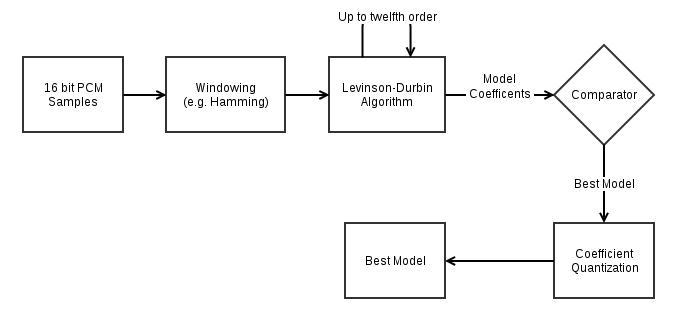
\includegraphics[scale=.8]{imgs/flac_lpc_overview}}
    \caption{Finding the best lpc model}
    \label{fig:lpc_optimisation}
  \end{figure}
  In the case of the Levinson-Durbin method, more effort is required. First, the input data must be windowed in order for it to be correctly modeled in the frequency domain. The window selected tends to have a significant effect on the quality of the resulting model, so it must be chosen carefully. The autocorrelation of the windowed data is then calculated. Next, the Levinson-Durbin algorithm is used to find the model coefficients for orders from the minimum to the maximum order (the fLaC specification allows up to twelfth order predictors\cite{flac_format}). The total absolute error is then calculated for each model similar to the fixed method, and the optimum model is selected. The encoder must then quantise the model coefficients, since the Levinson-Durbin method produces floating point coefficients.
  
  \subsubsection*{Finding the best entropy encoding}
  \begin{figure}[H]
    \centering{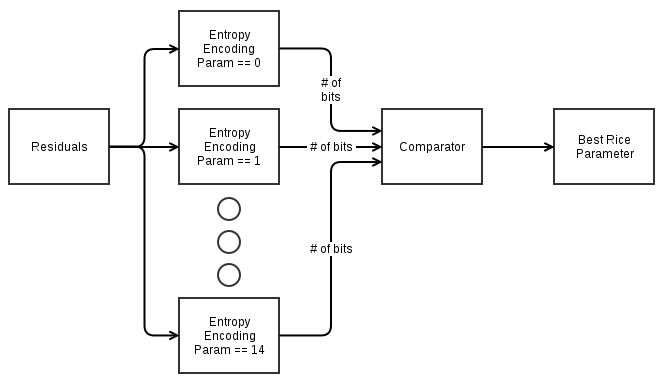
\includegraphics[scale=.8]{imgs/flac_entropy_overview.png}}
    \caption{Finding the best entropy coding}
    \label{fig:entropy_optimisation}
  \end{figure}
  Once the best linear predictor has been found, the encoder calculates the residuals (the difference between the model and the actual audio samples) and sends them through to the entropy encoder. Whilst there are a number of different entropy encoding methods available, including Huffman coding (used in JPEG\cite{jpeg_standard}), arithmetic coding, and Golomb codes, fLaC uses a subset of the Golomb codes known as Rice coding. Rice coding is used because it is very easy to implement on digital computers, as it consists only of bit shifts. The Rice coding method takes a binary number \(x\) and divides it by the rice parameter \(K\). The quotient is encoded in unary (\(n\) zeros followed by a one), and the remainder as K binary bits. The advantage of this method is that so long as the majority of the residuals are less than the rice parameter \(K\), a net reduction in encoded residual size will result. 
  
  In order to optimize the rice parameter for a particular stream of data, the fLaC algorithm allows the parameter to vary within a block of residuals. Each \textit{partition} within a block may have a different rice parameter, with as many partitions as there are residuals allowed.  A prefix sum algorithm is used to find the optimum combination of partition size and rice parameter allocation.
  
  \subsubsection*{Encoding and Framing} 
    \begin{figure}[H]
    \centering{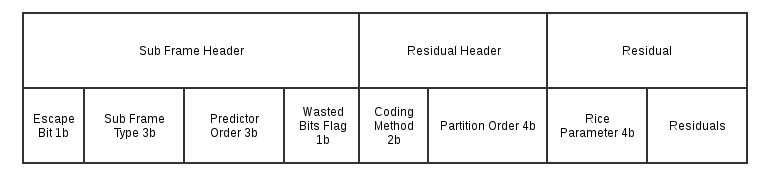
\includegraphics[scale=.8]{imgs/subframe_header.png}}
    \caption{Typical framing of a Subframe header}
    \label{fig:subframe_header}
  \end{figure}
  The final stage of the encoder is to encode and frame the audio data. The data is run through the best discovered model to produce the residuals. The residuals are then encoded using the best rice parameters. Finally, the resulting data, parameters, model coefficients, and audio file information (e.g. sample rate) is framed according to the fLaC format and written out to a file buffer, usually with significant compression having been achieved.
  
  \subsubsection{fLaC Decoding Process}
  \begin{figure}[H]
    \centering{\includegraphics[scale=.65]{imgs/fLaC_Format_Diagram.png}}
    \caption{fLaC Format Structure}
    \label{fig:flac_format_diagram}
  \end{figure}
  The decoding process for fLaC is fairly simple. The decoder first reads the fLaC stream's' metadata block, which gives the decoder important information. This includes the sample rate, bits per sample, number of frames in the stream, number of channels, and other pertinent information. Once the metadata has been processed, the decoder then begins the process of decoding each frame. \\
  
  The frame restates a subset of the data of the metadata block, this is so that the fLaC format can be streamed, as each frame can be decoded independently. After reading the frame metadata, the decoder then begins to decode each subframe. Each audio channel in the fLaC format is stored as consecutive subframes, rather than interleaved. This is so that interchannel decorrelation can be used. The subframe type is read from the subframe header, this can be either CONSTANT, VERBATIM, FIXED, or LPC. The constant type is used when all the audio samples within the block are identical, often this will happen in a section of audio that is silent. The verbatim type is used when no predictor provides any compression advantage, in very chaotic and unpredictable pieces of audio this may occur. The fixed type describes an audio block encoded using predetermined (or fixed) prediction coefficients, and the LPC type describes an audio block encoded using optimally determined prediction coefficients, which are given in the header. \\
      
  Once the type of subframe has been determined, the decoder simply decodes the following residual, and applies the given linear predictor to recover the original signal. This is a fairly straightforward process which consists only of integer operations.
  
  \section{Project Requirements}
  \subsection{Goals}
  The goal of this project is to explore the implementation of a fLaC decoder and encoder targetting an FPGA platform. Major requirements are listed below.
  \begin{itemize}
    \item Implement a fLaC compatible encoder in C++.
    \item Implement a fLaC compatible decoder in C++.
    \item Implement a fLaC compatible encoder in Verilog.
    \item Implement a fLaC compatible decoder in Verilog.
    \item Identify areas of the encoding process that can be accelerated using FPGA hardware.
    \item Identify areas of the decoding process that can be accelerated using FPGA hardware.
    \item Optimize the fLaC encoder in the areas identified.
    \item Optimize the fLaC decoder in the areas identified.
  \end{itemize}
  
  \subsection{Changes to original requirements}
  Whilst the original requirements specified a fully fLaC compatible encoder and decoder, I have decided to reduce the goal to a subset of the fLaC specification. The new target is to decode and encode single channel 16 bit fLaC files. Whilst it would not be a major leap to add stereo support, I believe that there is little to be gained from an academic perspective by doing so and would prefer to limit the problem domain in order to focus on the more interesting areas of optimizing the decoder and encoder, rather than concern myself with implementing extraneous features.\\
      
  Similarly, the project will not focus on producing an implementation to run on an FPGA, although it would be a nice artefact, the main goal is to investigate and implement the opportunities for optimization.
      
  The main target of the optimization has also shifted. Whilst it was originally planned to optimize both the decoder and the encoder, I have decided to focus my efforts on the encoder for a number of reasons. Firstly, the encoder is the more computationally expensive part of the process, so it makes more sense to optimize that. Real time software decoding of fLaC is already possible, so optimizing the decoder is not as pressing an issue. The encoder also has some more interesting opportunities for improvement. For example, the Levinson-Durbin algorithm as implemented in the fLaC reference implementation uses floating point operations. It would be interesting to see whether this process could be changed to use fixed point operations instead. Encoding of the residuals lends itself to large parallel computations, perfect for an FPGA. Overall, the encoding process is the more interesting component, and thus will be the focus of next semester's work.
  
  \section{Conclusion}
  The goals of this project have changed somewhat from the original plan. The project will focus much more on optimizing the encoder, and perhaps even focusing on one small subset of it. The fLaC format provides many opportunities for optimization and investigation into hardware acceleration techniques on FPGAs.
  
  \bibliography{references}
  
\end{document}
